\clearpage
\subsection{Statement (with Assignment)} % (fold)
\label{sub:statement_with_assignment_}

Statements are the actions that we can get the computer to perform. At this stage we have covered the statements that run procedures, the \nameref{sub:procedure call}, and the statement to assign values to variables, the \nameref{sub:assignment_statement}.

\begin{figure}[h]
   \centering
   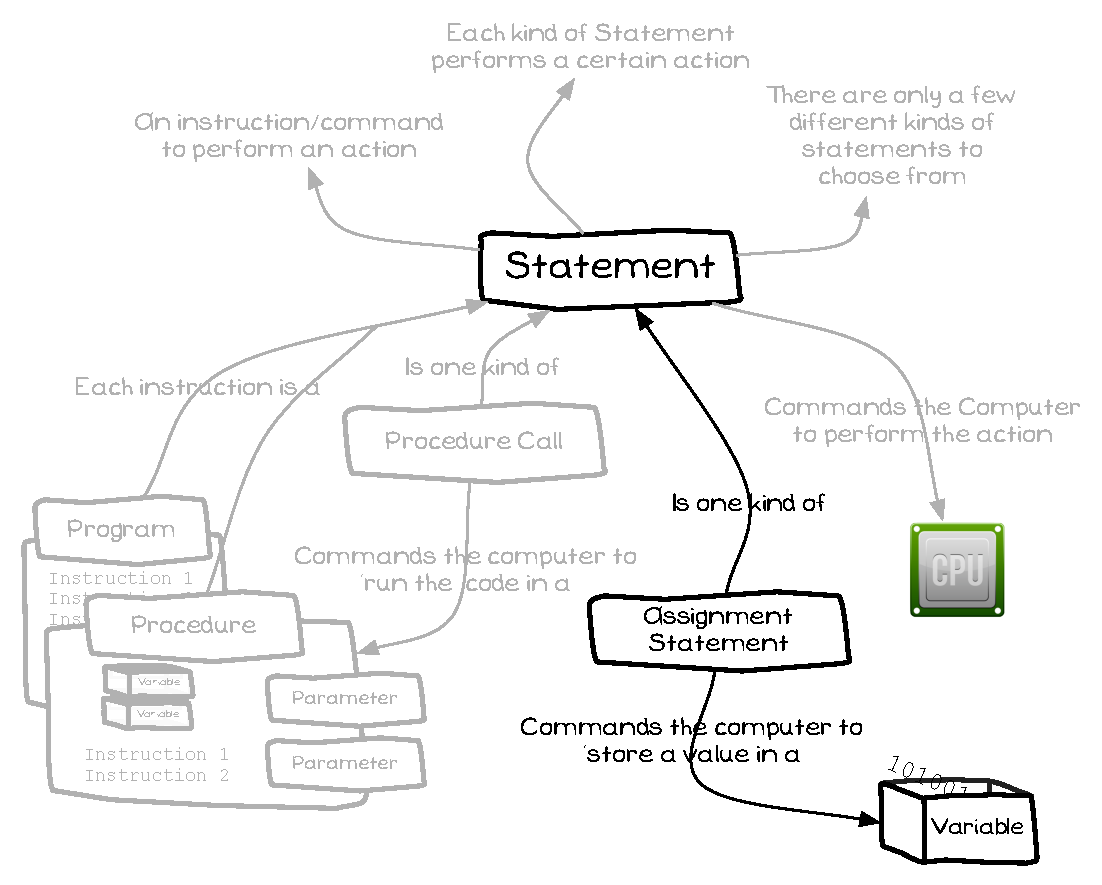
\includegraphics[width=\textwidth]{./topics/storing-using-data/diagrams/Statement} 
   \caption{A Statement may be an Assignment statement}
   \label{fig:storing-using-data-statement}
\end{figure}

\mynote{
\begin{itemize}
  \item Statement is the \textbf{term} given to the instructions in our code.
  \item Statements can be either:
  \begin{itemize}
    \item \nameref{sub:procedure call} used to run the code in a Procedure, as covered in Chapter \ref{cha:program_creation}.
    \item \nameref{sub:assignment_statement} used to calculate a value and store it in a Variable.
  \end{itemize}
  \item All instructions in your code are Statements, these include the instructions in your Program as well as the instructions in your Procedures and Functions.
\end{itemize}
}

% subsection statement_with_assignment_ (end)